% fig_freq_adaptive_block.tex
% Block diagram: frequency-adaptive 87L processing pipeline (TR-20)
% Stages: voltage measurement → freq est → adaptive B_C → LM estimator → trip
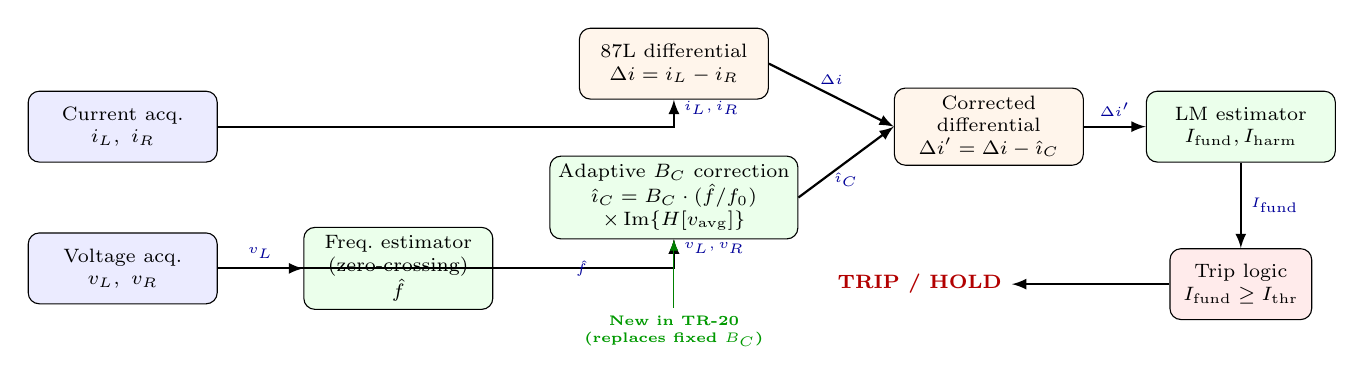
\begin{tikzpicture}[
  blk/.style={draw, rounded corners=4pt, fill=blue!8,
              minimum width=2.4cm, minimum height=0.9cm,
              font=\scriptsize, align=center, inner sep=3pt},
  blk2/.style={draw, rounded corners=4pt, fill=green!8,
               minimum width=2.4cm, minimum height=0.9cm,
               font=\scriptsize, align=center, inner sep=3pt},
  blk3/.style={draw, rounded corners=4pt, fill=orange!8,
               minimum width=2.4cm, minimum height=0.9cm,
               font=\scriptsize, align=center, inner sep=3pt},
  blkr/.style={draw, rounded corners=4pt, fill=red!8,
               minimum width=1.8cm, minimum height=0.9cm,
               font=\scriptsize, align=center, inner sep=3pt},
  arr/.style={-latex, thick},
  sig/.style={font=\tiny\itshape, blue!60!black},
]

% ---- Inputs ----------------------------------------------------------------
\node[blk]  (iacq)  at (0, 1.2)
  {Current acq.\\$i_L,\ i_R$};
\node[blk]  (vacq)  at (0, -0.6)
  {Voltage acq.\\$v_L,\ v_R$};

% ---- Frequency estimator ---------------------------------------------------
\node[blk2] (fest)  at (3.5, -0.6)
  {Freq.\ estimator\\(zero-crossing)\\$\hat{f}$};
\draw[arr] (vacq.east) -- node[above, sig]{$v_L$} (fest.west);

% ---- Adaptive charging correction ------------------------------------------
\node[blk2] (corr)  at (7.0, 0.3)
  {Adaptive $B_C$ correction\\$\hat{\imath}_C = B_C \cdot (\hat{f}/f_0)$\\$\times\,\mathrm{Im}\{H[v_{\rm avg}]\}$};
\draw[arr] (vacq.east) -| node[right, sig, pos=0.85]{$v_L, v_R$}
  (corr.south);
\draw[arr] (fest.east)  -| node[right, sig, pos=0.20]{$\hat{f}$}
  (corr.south);

% ---- Differential computation ----------------------------------------------
\node[blk3] (diff)  at (7.0, 2.0)
  {87L differential\\$\Delta i = i_L - i_R$};
\draw[arr] (iacq.east) -| node[right, sig, pos=0.85]{$i_L, i_R$}
  (diff.south);

% ---- Corrected differential ------------------------------------------------
\node[blk3] (cdiff) at (11.0, 1.2)
  {Corrected\\differential\\$\Delta i' = \Delta i - \hat{\imath}_C$};
\draw[arr] (diff.east)  -- node[above, sig]{$\Delta i$} (cdiff.west);
\draw[arr] (corr.east)  -- node[below, sig]{$\hat{\imath}_C$} (cdiff.west);

% ---- LM estimator ----------------------------------------------------------
\node[blk2] (lm)    at (14.2, 1.2)
  {LM estimator\\$I_{\rm fund}, I_{\rm harm}$};
\draw[arr] (cdiff.east) -- node[above, sig]{$\Delta i'$} (lm.west);

% ---- Trip decision ---------------------------------------------------------
\node[blkr] (trip)  at (14.2, -0.8)
  {Trip logic\\$I_{\rm fund} \geq I_{\rm thr}$};
\draw[arr] (lm.south) -- node[right, sig]{$I_{\rm fund}$} (trip.north);
\draw[arr] (trip.west) -- ++(-2.0, 0)
  node[left, font=\scriptsize\bfseries, red!70!black]{TRIP / HOLD};

% ---- Label: new block ------------------------------------------------------
\node[font=\tiny\bfseries, green!60!black, align=center]
  at (7.0, -1.4) {New in TR-20\\(replaces fixed $B_C$)};
\draw[-latex, green!50!black, thin]
  (7.0, -1.1) -- (corr.south);

\end{tikzpicture}
